\documentclass[12pt]{article}
\usepackage{fullpage,tikz,graphicx}


\usetikzlibrary{automata ,positioning, arrows}


\title{CS 360: Assignment 3}
\author{Cam J. Loader}

\begin{document}
\maketitle

\begin{enumerate}

\item  (10 points) Let the language L be the set of strings on Σ = {a; b} such that the number of
occurrences of a is five more than the number of occurrences of b. Use the pumping lemma
to prove that L is not a regular language. Write your proof in regular English sentences and
paragraphs.

Let L be a language on {a,b} such that $a^{5n}b^n$ holds. We are going to use a proof by contradiction to prove that L is not a regular language. Using the pumping lemma, we can break up $a^{5n}b^n$ into u, v, w and demonstrate three cases hold. If we cannot, tgen it will not be a regular laqnguage.

Suppose we have a string  $x$ such that:
$$x = a^{5n}b^n$$ and we can break up the string into u,v,w such that:

(i.) x =uvw

(i.) v is not empty

(iii.) $|uv|>n $ where n is in the pumping lemma.


Lets choose n=2, $a^{5*2}b^2$. aaaaaaaaaabb is part of L. Lets choose n = 3, aaaaaaaaaaaaaaaaaabbb is part of L.

(Not sure how to proceed from here)

\item 

Leftmost Derivation:

\begin{tabular}{| c | c | c| c|}
    \hline
    Step & Production & Current Expression & New Expression \\ \hline \hline
    1 & $E -> E/E$ & $E$ & $E/E $\\
    2 & $E -> (E)$ & $E/E $& $(E)/E$ \\
    3 & $E -> E+E$ & $(E)/E $& $(E+E)/E$ \\
    5 & $E -> n$ & $(E+E)/E $& $(n+E)/E$ \\
    6 & $E -> n$ & $(n+E)/E $& $(n+n)/E$ \\
    7 & $E -> n$ & $(n+n)/E $& $(n+n)/n$ \\
\hline
\end{tabular}

Rightmost Derivation:

\begin{tabular}{| c | c |c| c|}
\hline
    Step & Production & Current Expression & New Expression \\ \hline \hline
    1 & $E -> E/E$ & $E$ & $E/E $\\
    2 & $E -> n$ & $E/E $& $E/n$ \\
    3 & $E -> (E)$ & $E/n $& $(E)/n$ \\
    2 & $E -> E+E$ & $(E)/n $& $(E+E)/n$ \\
    2 & $E -> n$ & $(E+E)/n $& $(E+n)/n$ \\
    2 & $E -> n$ & $(E+n)/n $& $(n+n)/n$ \\
\hline
\end{tabular}

\item See figures.


\item Extra Credit

b) Leftmost Derivation:

\begin{tabular}{| c | c | c| c|}
\hline
    Step & Production & Current Expression & New Expression \\ \hline \hline
    1 & $S -> $ if S & $S$ & if S\\
    2 & $S -> $ if S else S & if S & if if S else S \\
    3 & $S -> $exp & if if S else S& if if exp else S \\
    4 & $S -> $exp & if if exp else S & if if exp else exp \\
\hline
\end{tabular}

    \begin{figure}
        \centering
                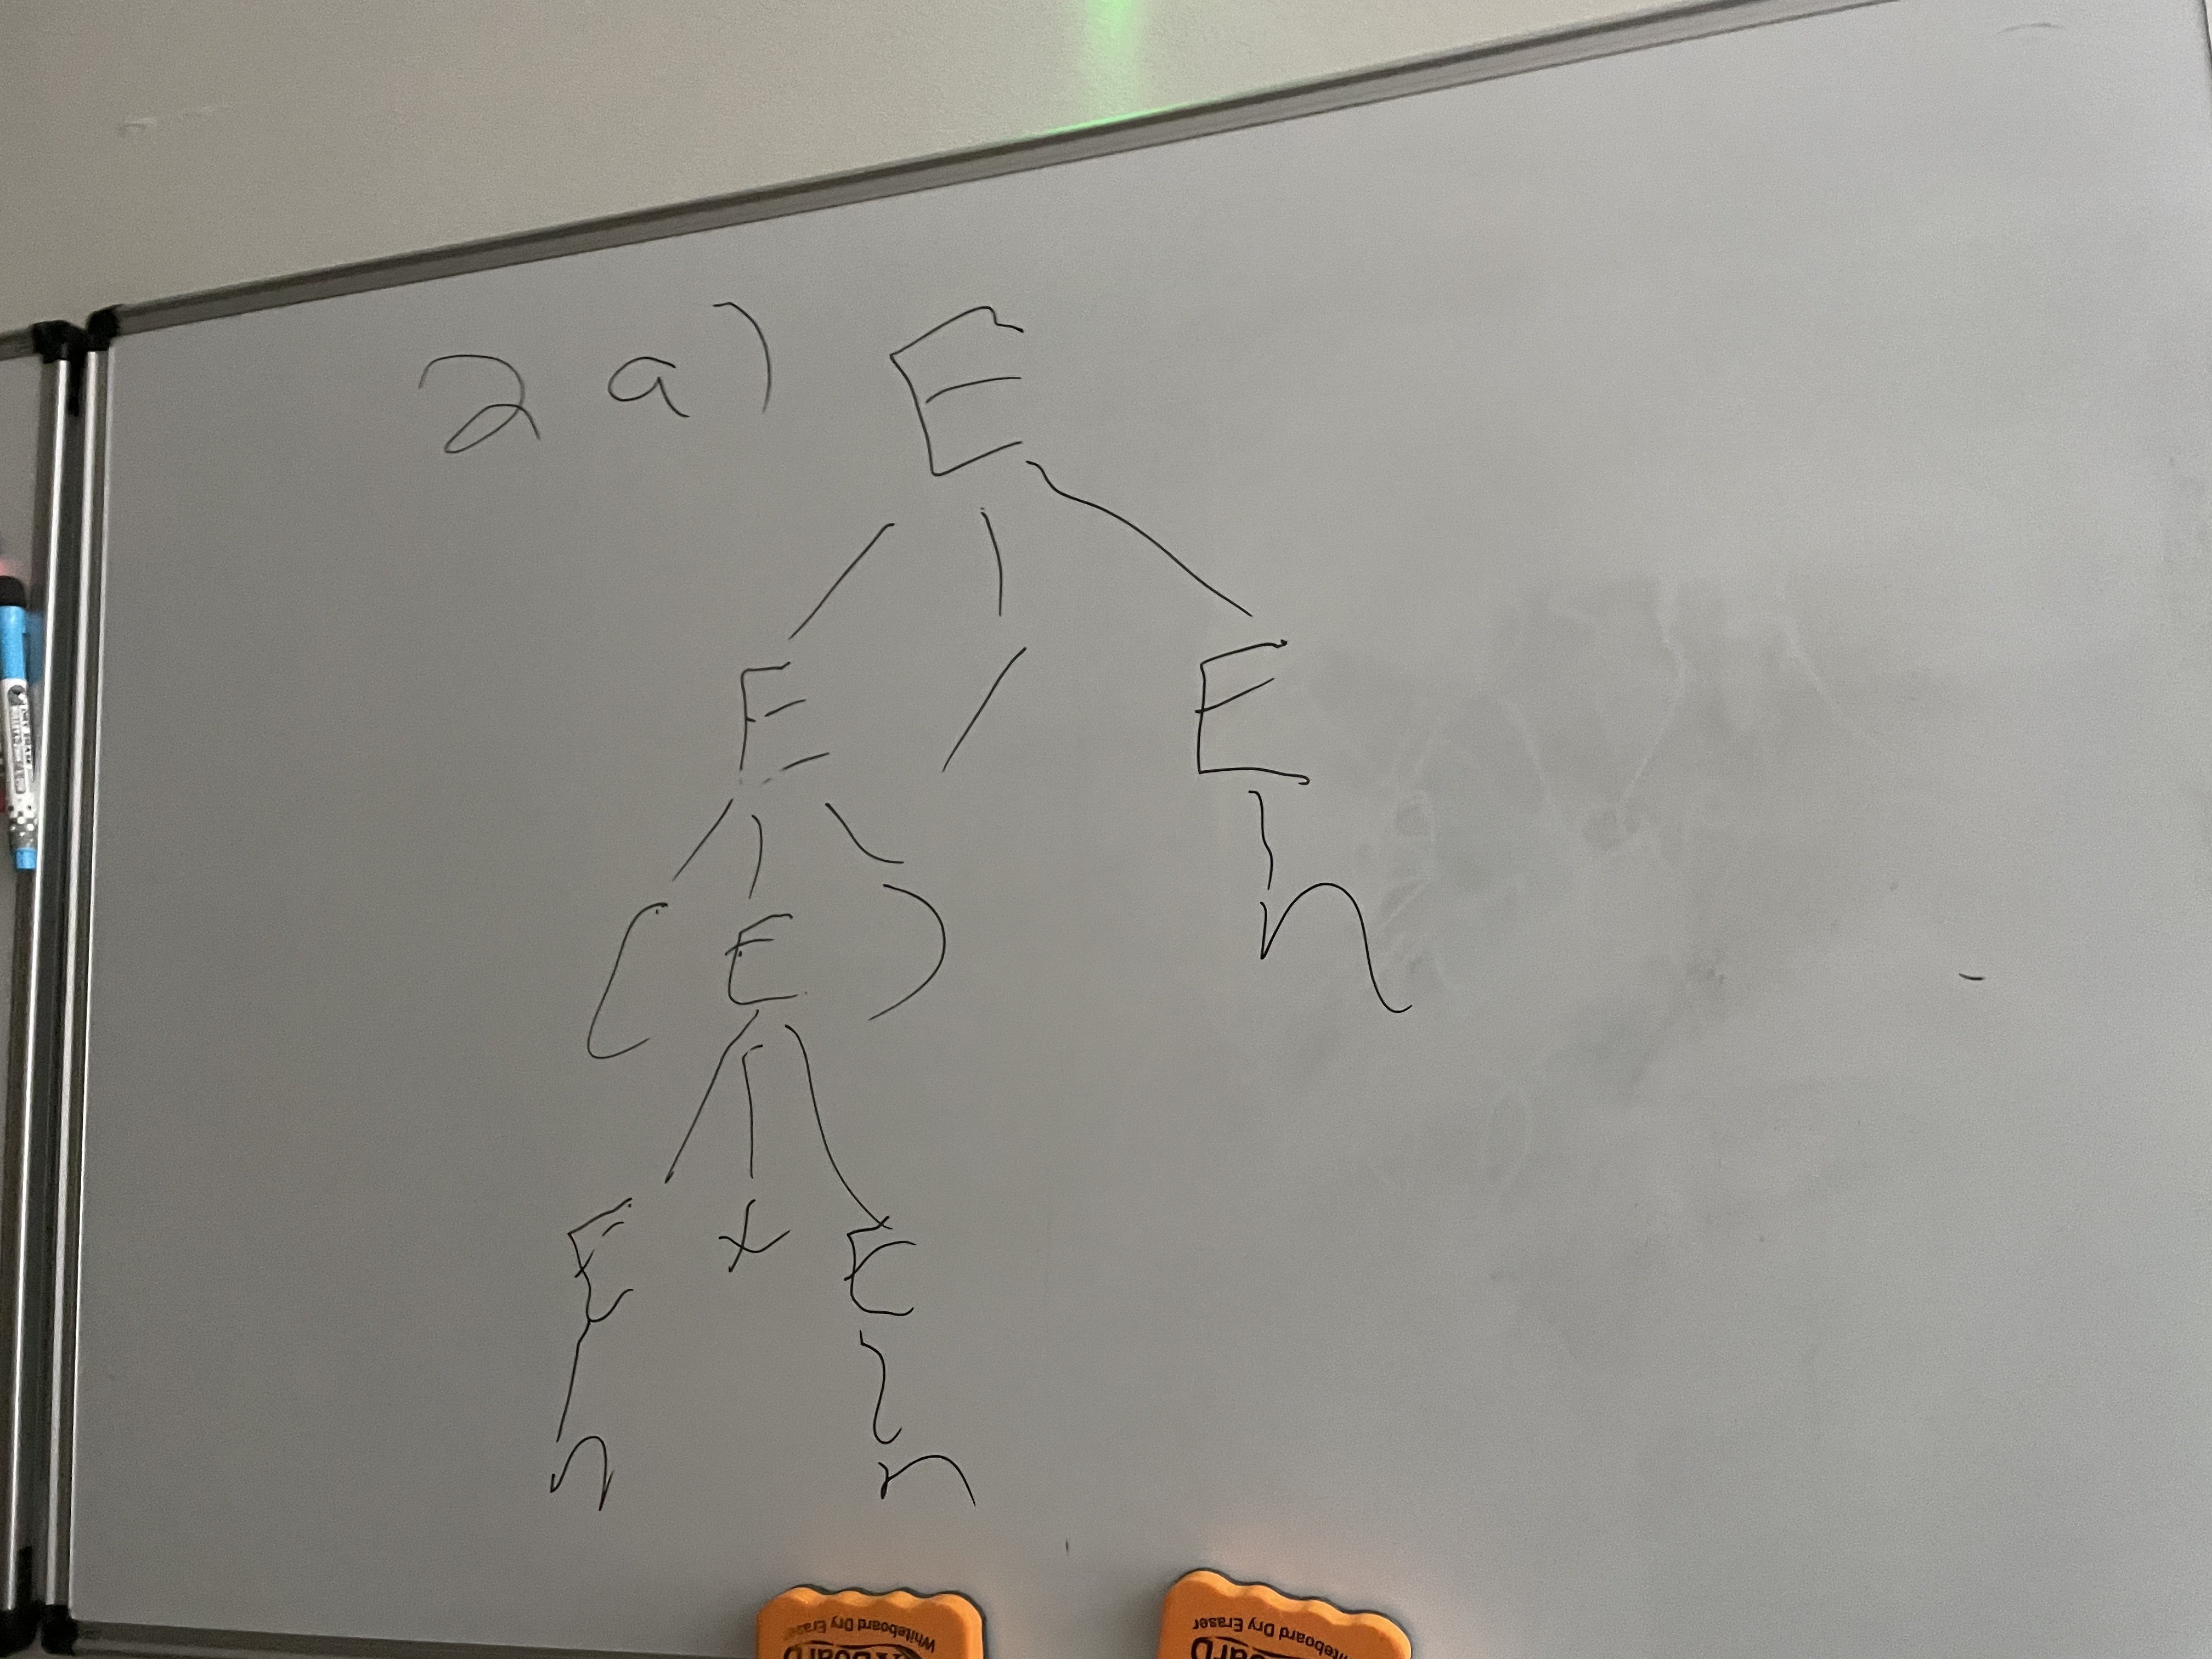
\includegraphics[totalheight=8cm]{2-a}
    \end{figure}
    \begin{figure}
        \centering
                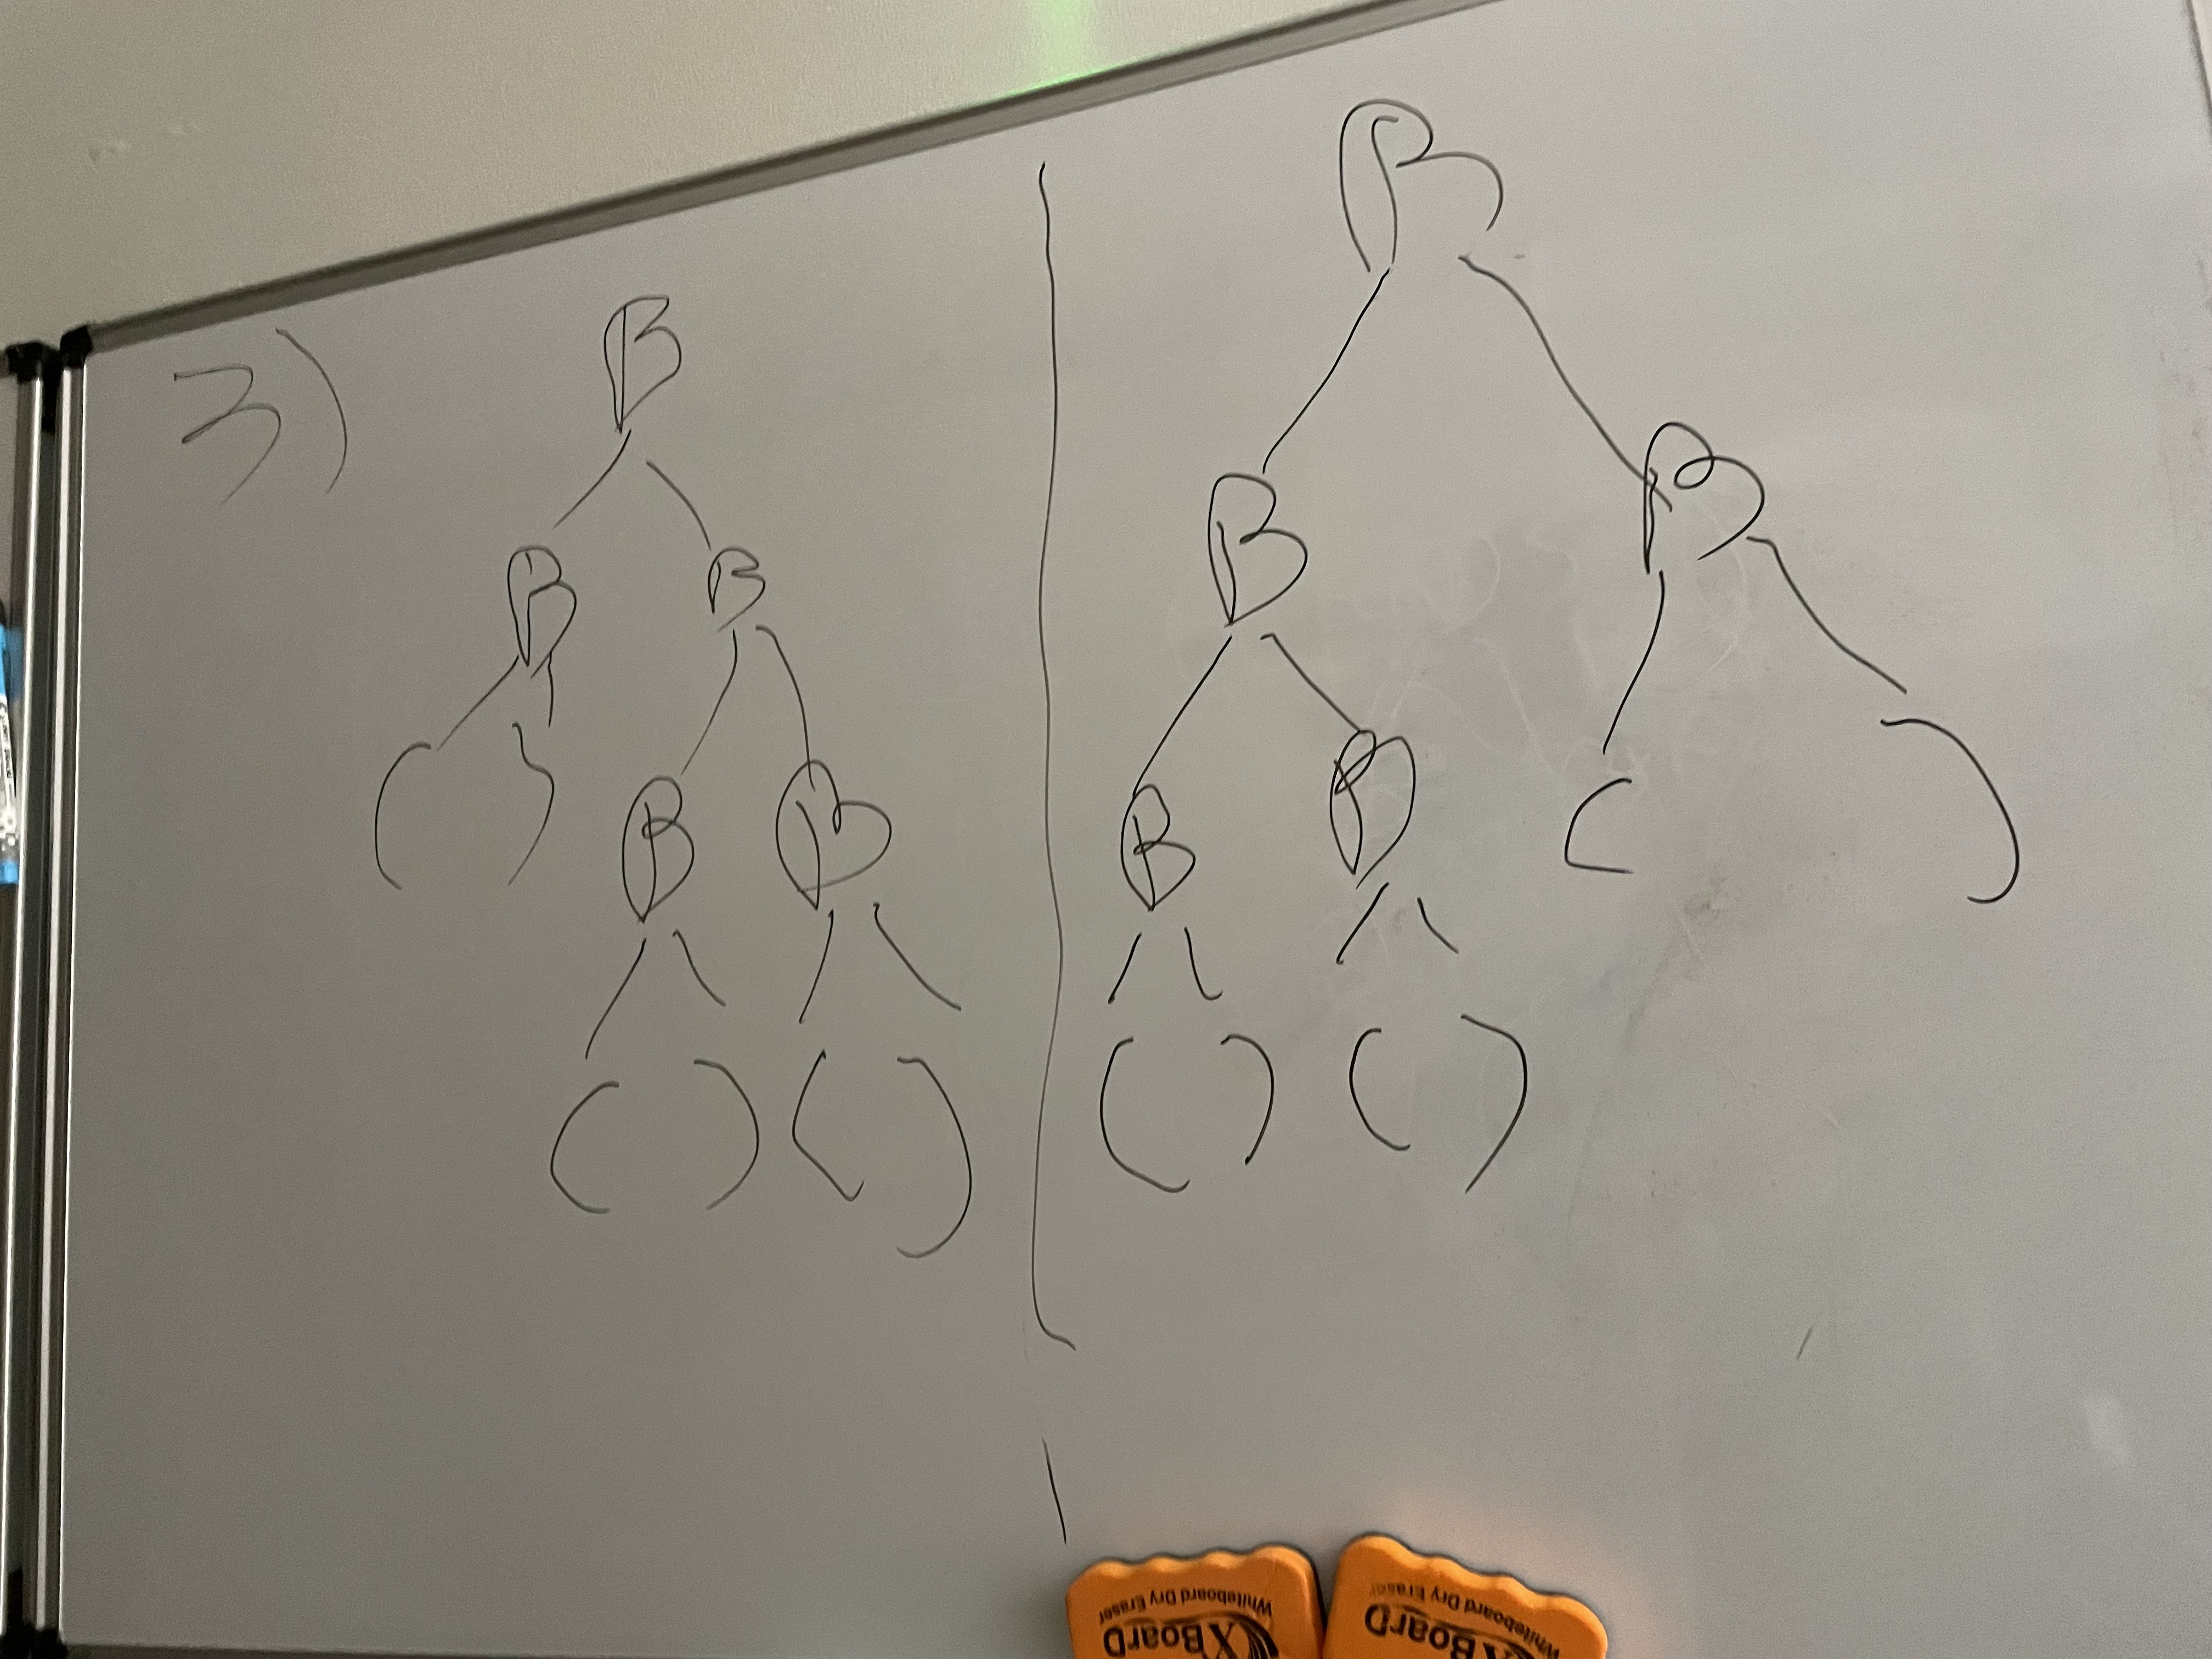
\includegraphics[totalheight=8cm]{3}
    \end{figure}
    \begin{figure}
            \centering
                    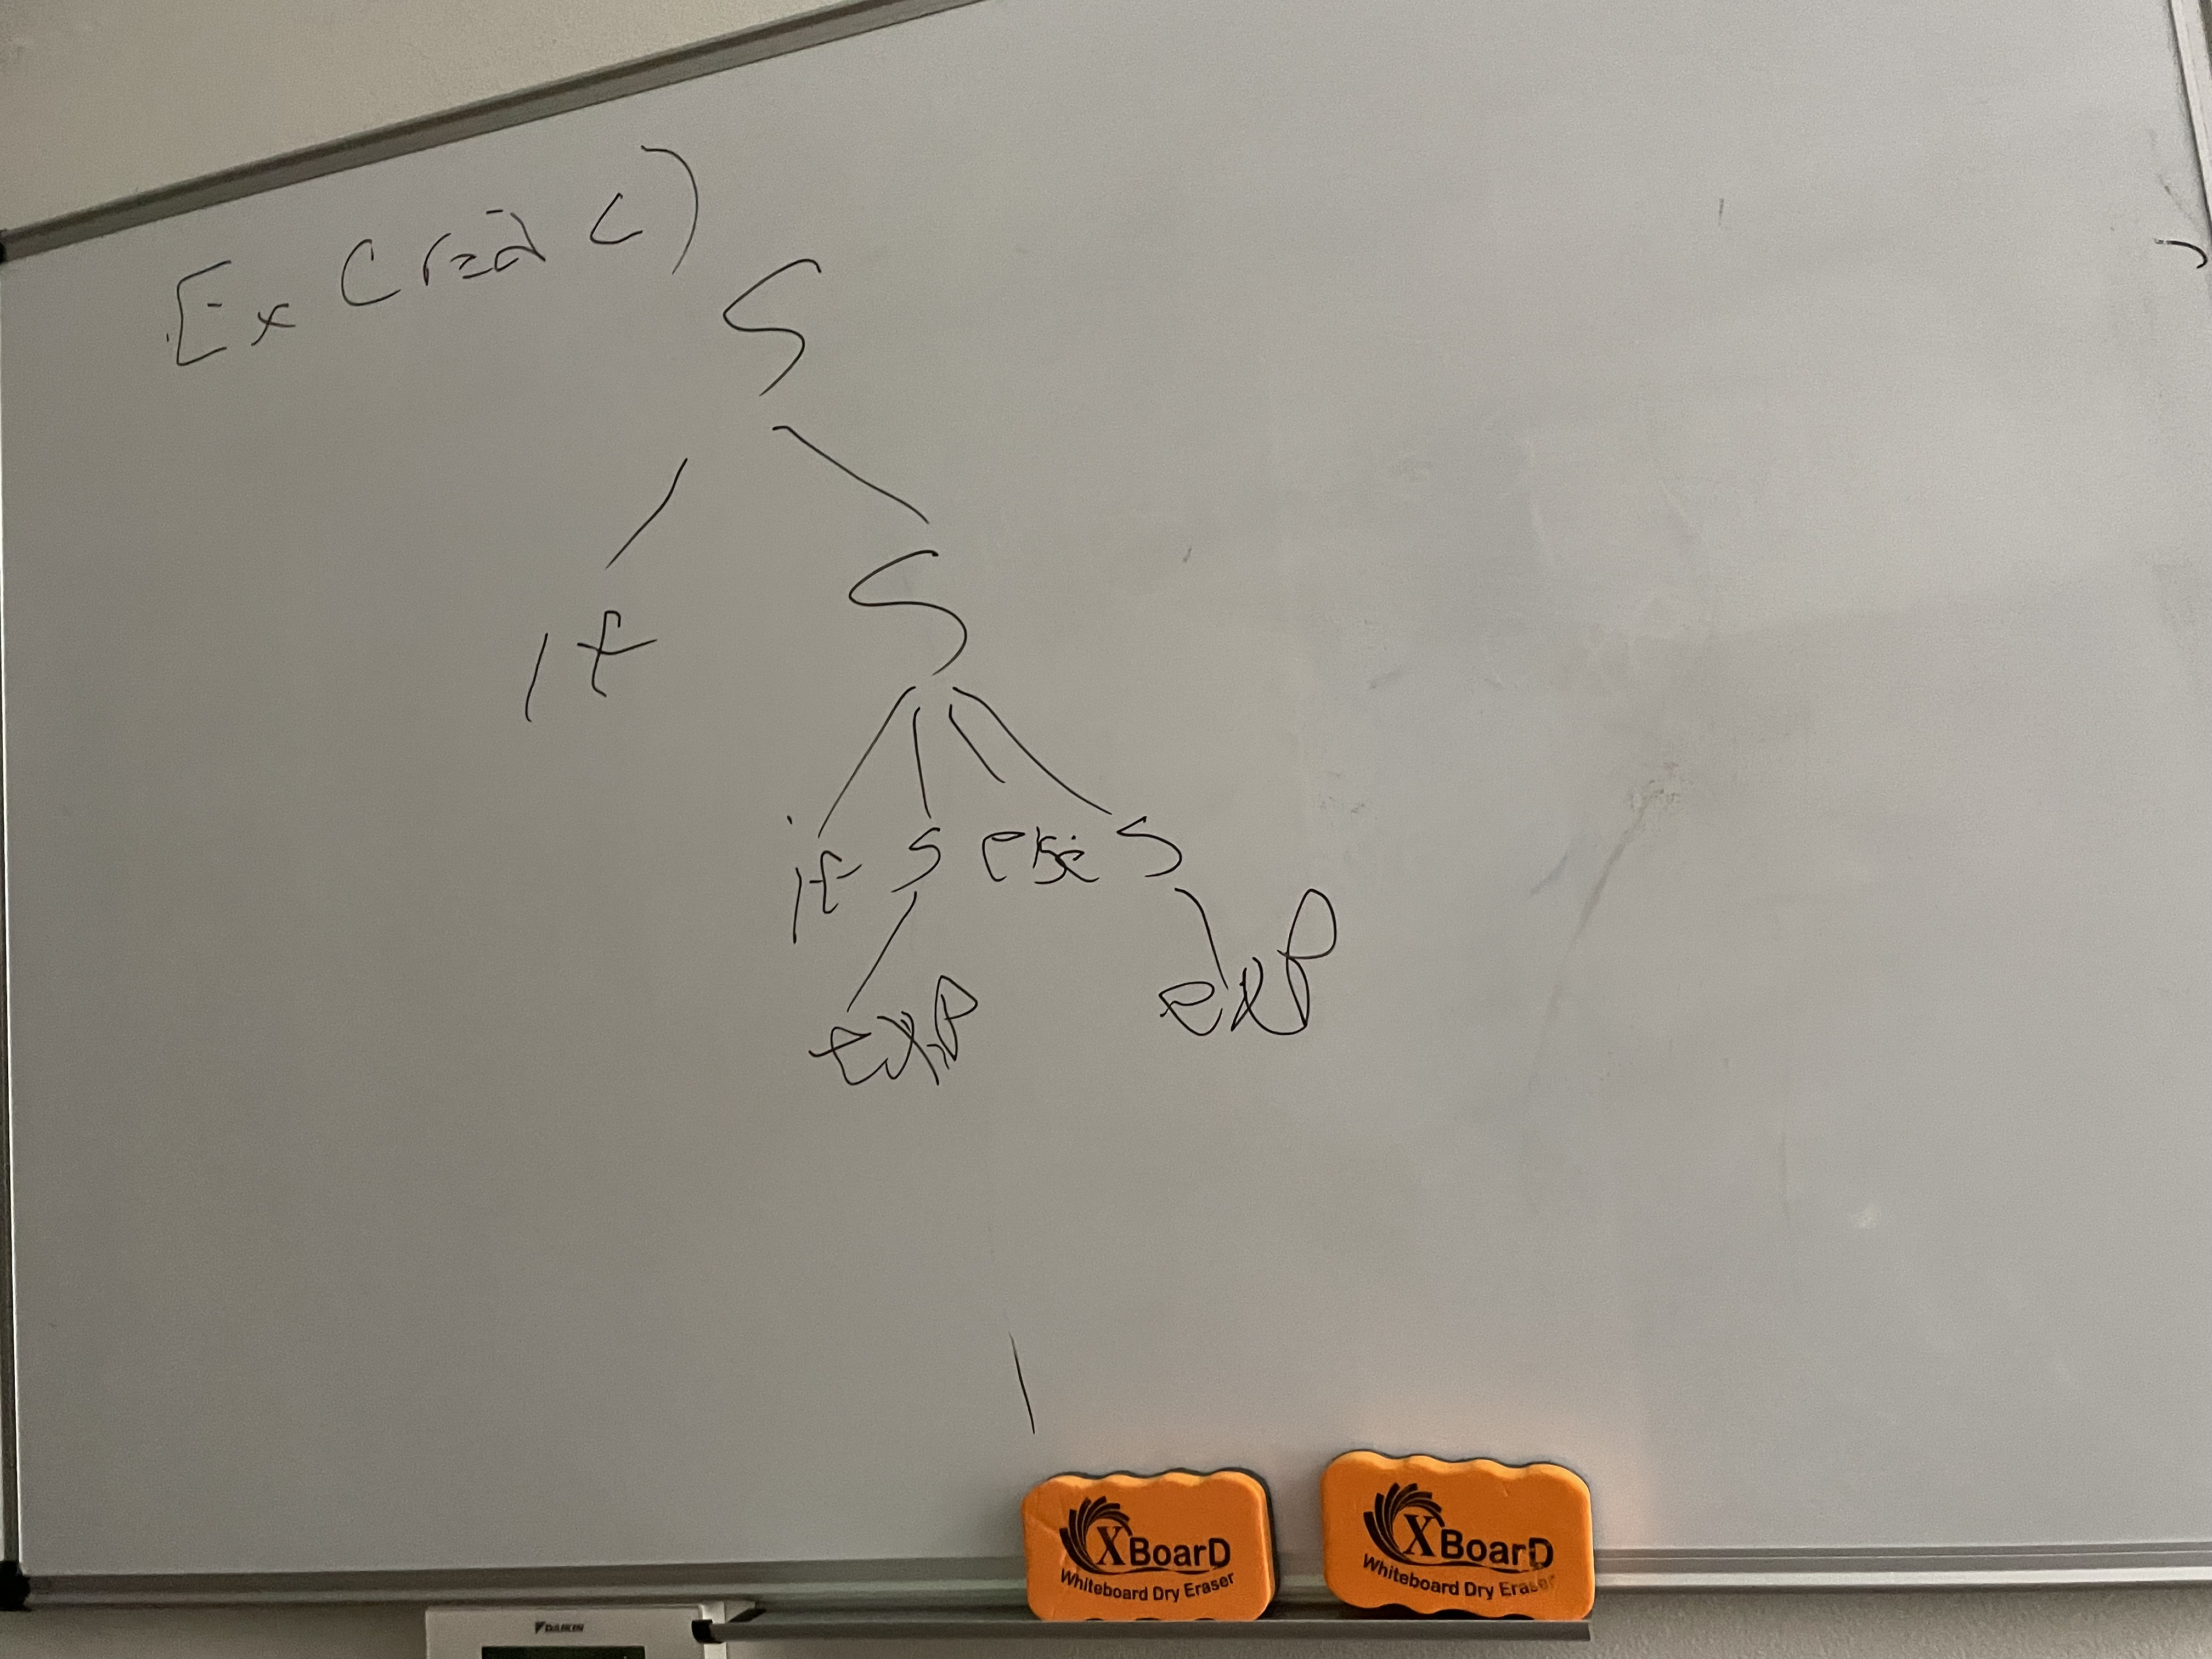
\includegraphics[totalheight=8cm]{ExCr-c}
    \end{figure}
    \begin{figure}
        \centering
                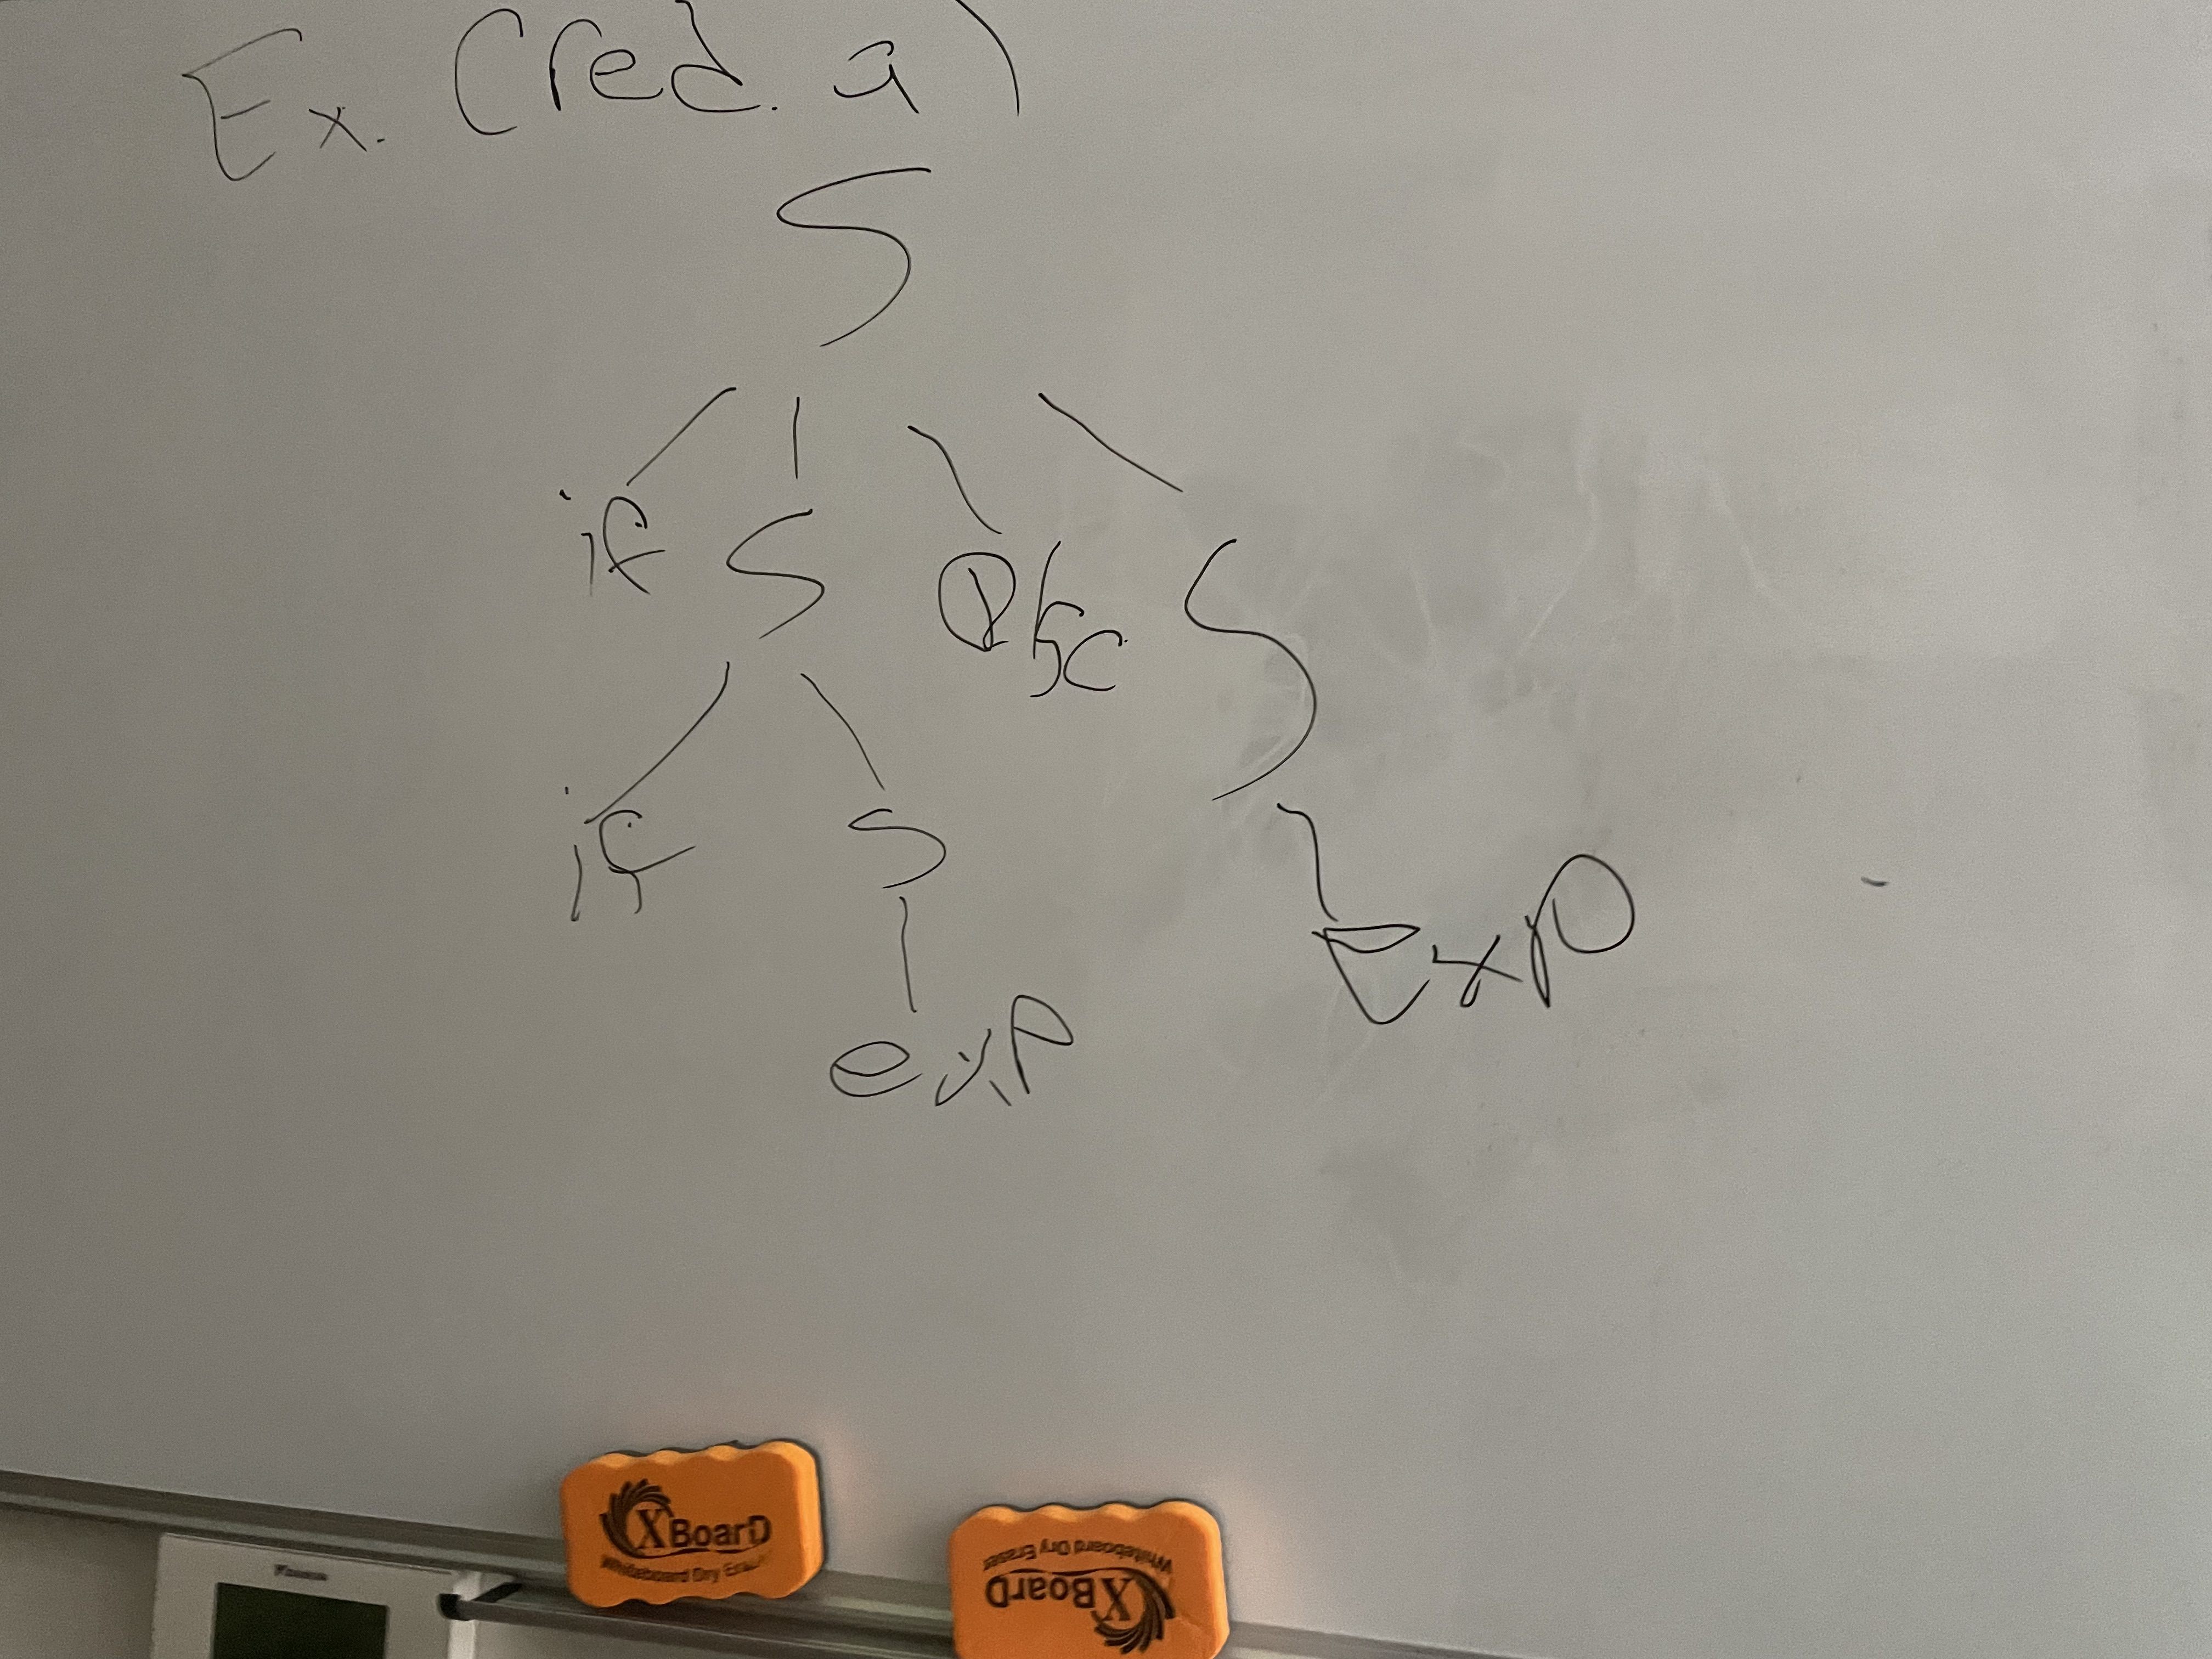
\includegraphics[totalheight=8cm]{ExCr-a}
    \end{figure}
    

\end{enumerate}

\end{document}